% 08 Appendix
\section{Appendices}

\subsection{Appendix A: Project Directory Structure}

Directory listing:
\begin{enumerate}
    \item Step_4_Detection/ - Main source code
    \begin{itemize}
        \item config/pipeline.yaml - Configuration
        \item gps\_monitor/ - MAVLink telemetry collector
        \item ml/ - Machine learning pipeline
        \item ui/ - Streamlit dashboard
    \end{itemize}
    \item tui/ - Terminal UI management
    \item gps\_logs/ - Data storage
    \item PX4-Autopilot/ - Flight stack
    \item run\_tui.py - Entry point
\end{enumerate}

\subsection{Appendix B: Configuration Files}

Central configuration in `Step_4_Detection/config/pipeline.yaml`:

\begin{lstlisting}[language=python, style=pythonstyle]
data:
  raw_dir: "gps_logs/raw"
  processed_dir: "gps_logs/processed"
  artifacts_dir: "ml/artifacts"
  models_dir: "ml/models"

cleaning:
  min_fix_type: 3
  max_dt_gap_s: 5.0

windows:
  length: 30    # 3 seconds @ 10Hz
  stride: 15      # 50% overlap

auto_label:
  enabled: true
  max_normal_speed_ms: 30.0
  min_satellites: 6
  max_eph_m: 5.0

training:
  model_type: "rf"
  n_estimators: 100

inference:
  connection_url: "udp:127.0.0.1:14560"
  anomaly_threshold: 0.5
\end{lstlisting}

\subsection{Appendix C: Commands Reference}

\begin{table}[htbp]
    \centering
    \caption{Command Reference}
    \label{tab:commands}
    \begin{tabular}{|p{4cm}|p{11cm}|}
        \hline
        \textbf{Command} & \textbf{Description} \\
        \hline
        python run\_tui.py & Start management interface (recommended) \\
        \hline
        python -m project.gps\_monitor.main & Run GPS monitor (MAVLink UDP) \\
        \hline
        python Step_4_Detection/ml/live\_inference.py & Run live anomaly detection \\
        \hline
        streamlit run Step_4_Detection/ui/app.py & Start dashboard (port 8501) \\
        \hline
        make px4\_sitl gz\_x500 & Start PX4 simulation in Gazebo \\
        \hline
        python -m project.ml.pipeline full & Run complete ML pipeline \\
        \hline
        python -m project.ml.pipeline process-batch & Process all raw logs \\
        \hline
        python -m project.ml.pipeline train & Train ML models only \\
        \hline
\end{tabular}
\end{table}

\begin{figure}[htbp]
    \centering
    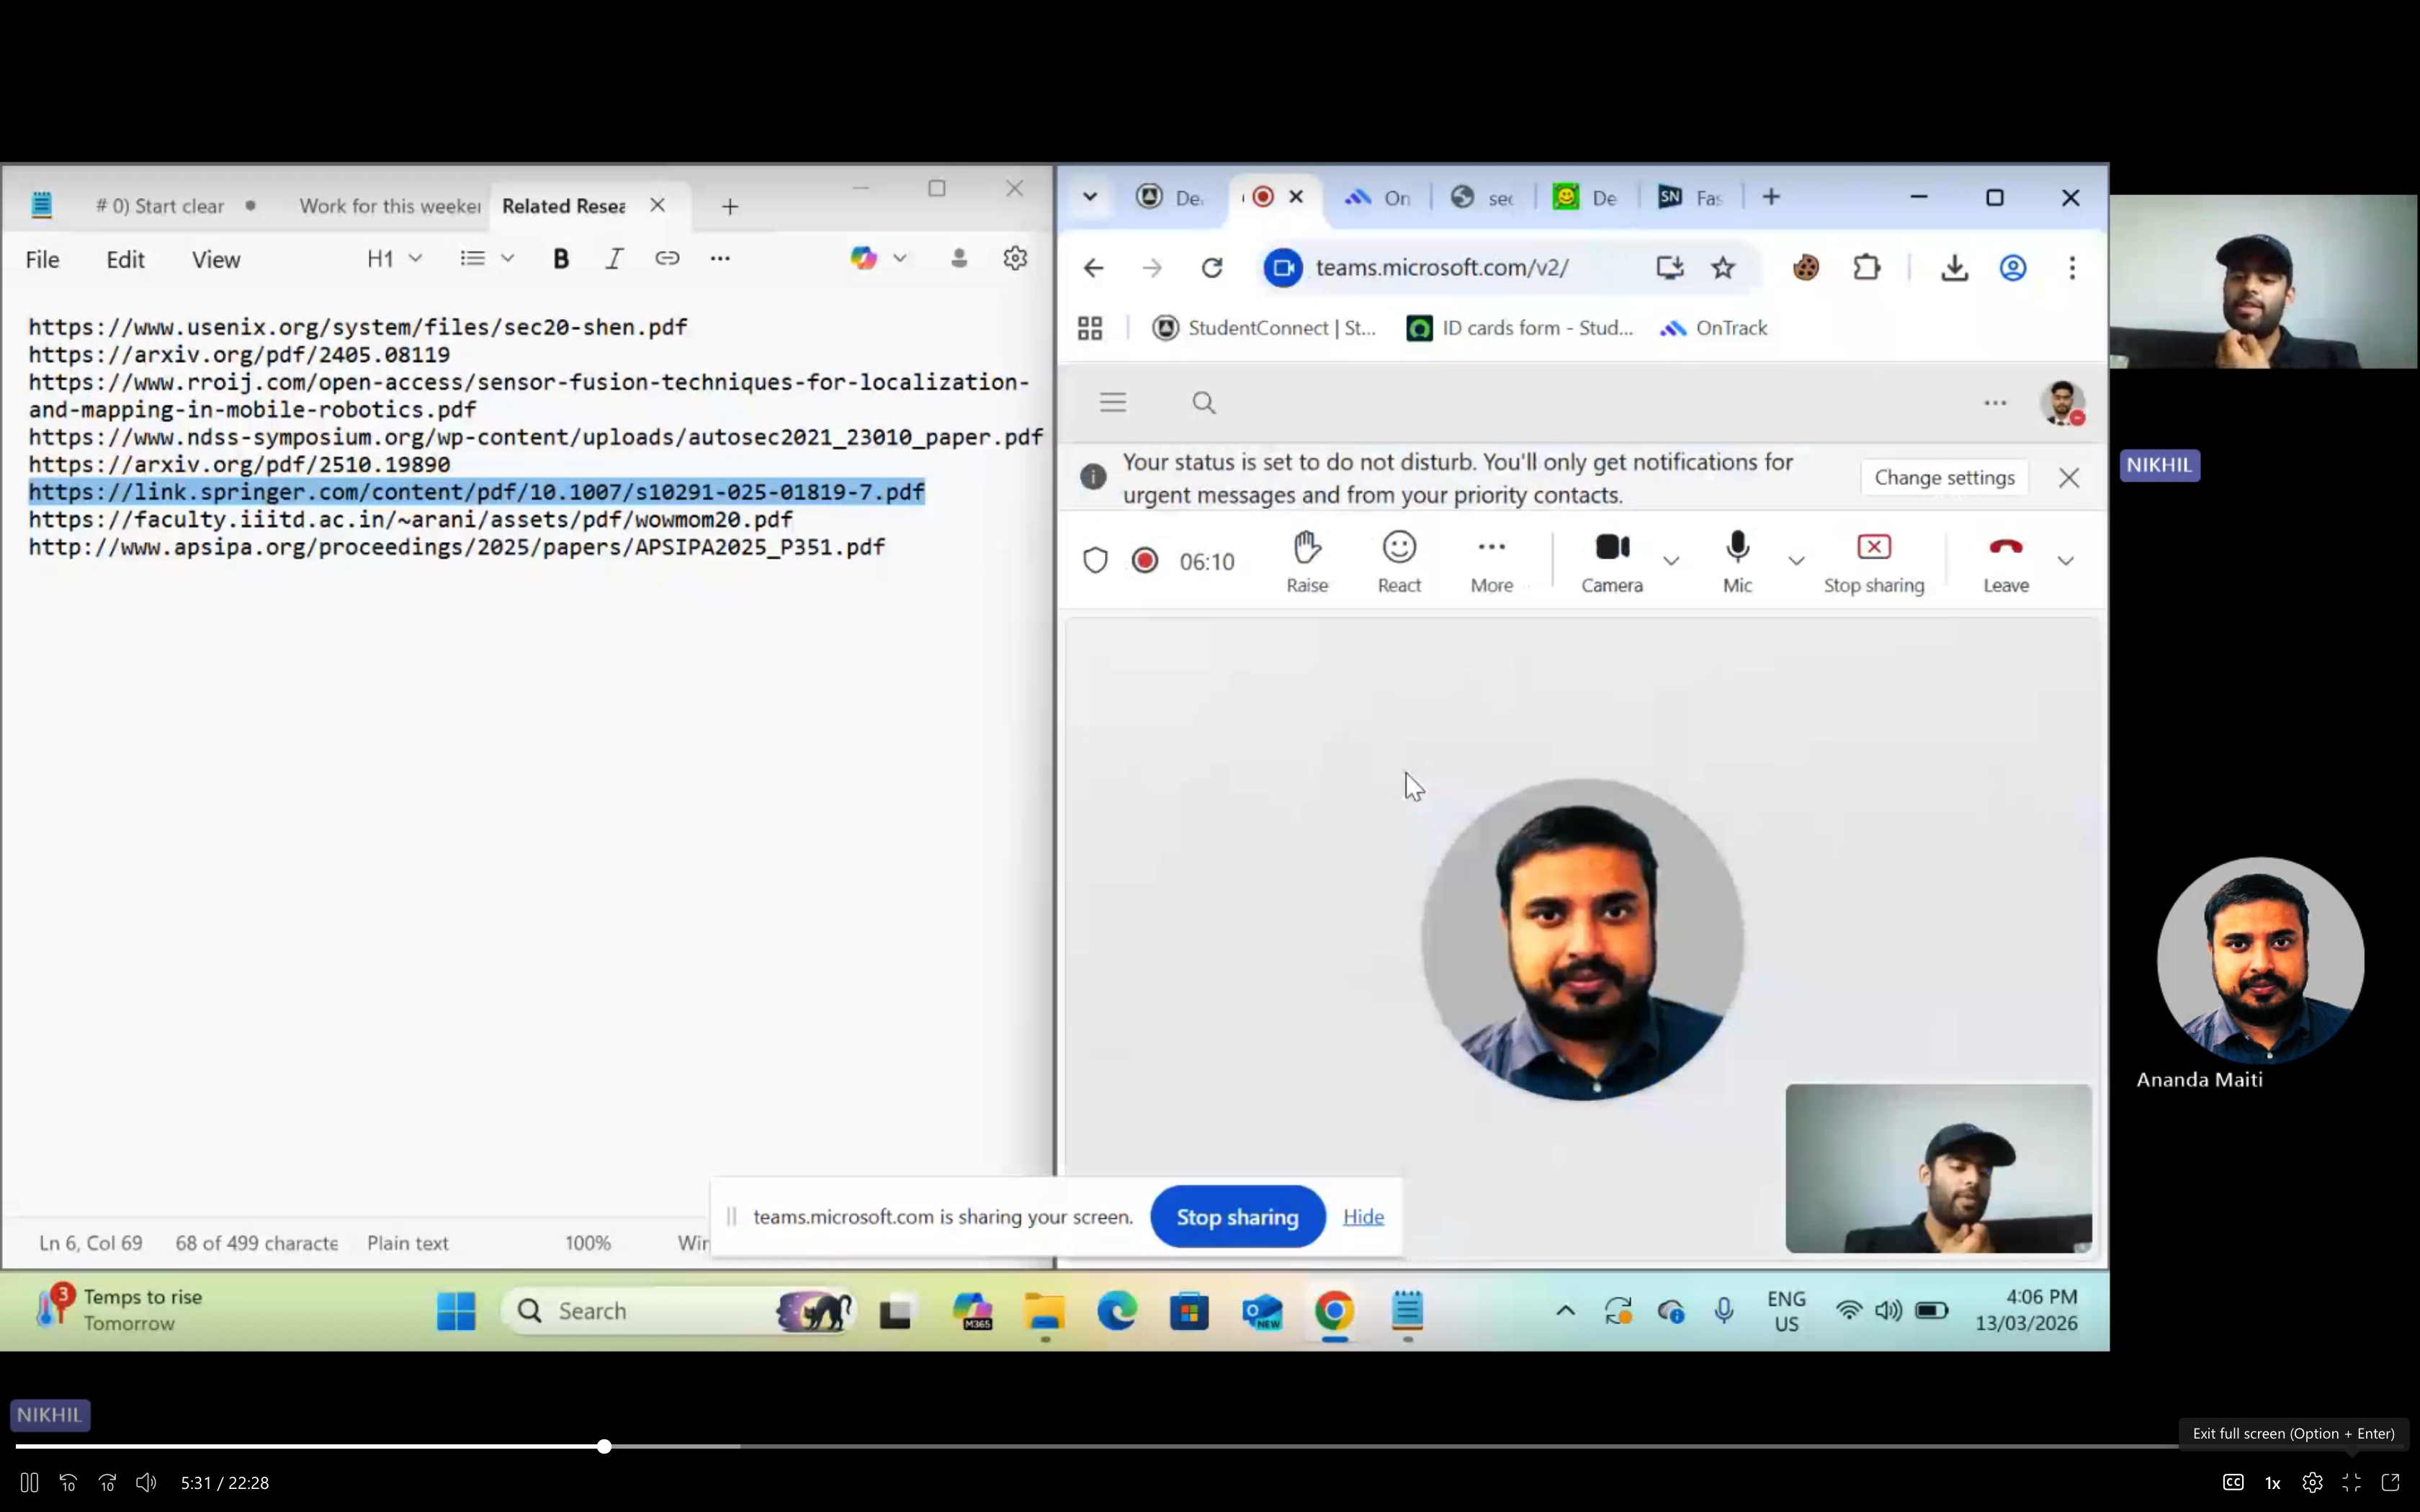
\includegraphics[width=0.6\linewidth]{figures/meeting first proof.png}
    \caption{Supervisor Meeting 1 - 13 March 2026}
    \label{fig:meeting1}
\end{figure}

\begin{thebibliography}{9}
    \bibitem{px4} PX4 Autopilot Documentation. \url{https://docs.px4.io/}
    \bibitem{mavlink} MAVLink Protocol Specification. \url{https://mavlink.io/}
    \bibitem{scikit} Scikit-learn: Machine Learning in Python. Pedregosa et al., JMLR 12, 2011.
    \bibitem{pytorch} PyTorch: An Imperative Style, High-Performance Deep Learning Library. Paszke et al., NeurIPS 2019.
    \bibitem{streamlit} Streamlit Documentation. \url{https://streamlit.io/}
\end{thebibliography}